\documentclass{article}
\usepackage[utf8]{inputenc}
\usepackage{amssymb}       % Librerías matemáticas
\usepackage{amsthm}        % Definición de teoremas
\usepackage{array}         % Nuevas características a las tablas
\usepackage{bigstrut}      % Líneas horizontales en tablas
\usepackage{bm}            % Caracteres en negrita en ecuaciones
\usepackage{booktabs}      % Permite manejar elementos visuales en tablas
\usepackage{caption}       % Leyendas
\usepackage{changepage}    % Condicionales para administrar páginas
\usepackage{chngcntr}      % Añade números a las leyendas
\usepackage{color}         % Colores
\usepackage{centernot}     % Flechas de cancelación
\usepackage{datetime}      % Fechas
\usepackage{enumitem}      % Listas con letras
\usepackage{floatpag}      % Maneja números de páginas
\usepackage{floatrow}      % Permite administrar posiciones en los caption
\usepackage{framed}        % Permite creación de recuadros
\usepackage{gensymb}       % Simbología común
\usepackage{graphicx}      % Propiedades extra para los gráficos
\usepackage{lipsum}        % Permite crear párrafos de prueba
\usepackage{listings}      % Permite añadir código fuente
\usepackage{longtable}     % Permite utilizar tablas en varias hojas
\usepackage{mathtools}     % Permite utilizar notaciones matemáticas
\usepackage{multicol}      % Múltiples columnas
\usepackage{needspace}     % Maneja los espacios en página
\usepackage{pdflscape}     % Modo página horizontal de página
\usepackage{pdfpages}      % Permite administrar páginas en pdf
\usepackage{physics}       % Paquete de matemáticas
% \usepackage{ragged2e}    % Redefine centering
\usepackage{rotating}      % Permite rotación de objetos
\usepackage{selinput}      % Compatibilidad con acentos
\usepackage{setspace}      % Cambia el espacio entre líneas
\usepackage{soul}          % Permite subrayar texto
\usepackage{subfig}        % Permite agrupar imágenes
\usepackage{textcomp}      % Simbología común
\usepackage{url}           % Permite añadir enlaces
\usepackage{wrapfig}       % Posición de imágenes
\usepackage{xspace}        % Adminsitra espacios en párrafos y líneas
\usepackage{amsmath}
%\usepackage{tikz}
\usepackage{mathdots}
\usepackage{yhmath}
\usepackage{cancel}
\usepackage{siunitx}
\usepackage{multirow}
\usepackage{tabularx}
\usepackage{xstring}
\usepackage[spanish,british]{babel}
\usepackage{hyperref}
\hypersetup{
    colorlinks=true,
    linkcolor=blue,
    filecolor=magenta,      
    urlcolor=cyan
}
%\usetikzlibrary{fadings}
%\usetikzlibrary{patterns}
%\usetikzlibrary{shadows.blur}
%\usetikzlibrary{shapes}

%-\hyperlink{label}{link}
%    -\hypertarget{label}{target}

% ------ CONFIG -------

\setlength{\parindent}{0pt} % Hace que los parrafos empiecen pegados a la izquierda

% Derivada parcial
% Modo de uso: \parfrac{ Función a derivar }{ Variable c/r a que se deriva }
\newcommand{\parfrac}[2]{\frac{\partial #1}{\partial #2}}

% Mantener constante variable #1
% Modo de uso: \mcte{ variable constante }{ derivada parcial }
\newcommand{\mcte}[2]{\left( #2 \right)_{#1}}

% Paréntesis grandes en comando 
% Modo de uso: \lados{ tipo de parentésis }{ Ecuación }
\newcommand{\lados}[2]{%
    \IfEqCase{#1}{%
        {(}{\left( #2 \right)}%
        {)}{\left( #2 \right)}%
        {()}{\left( #2 \right)}%
        {[}{\left[ #2 \right]}%
        {]}{\left[ #2 \right]}%
        {[]}{\left[ #2 \right]}%
        {\{}{\left\{ #2 \right\}}%
        {\}}{\left\{ #2 \right\}}%
    }[\PackageError{lados}{Opción no definida: #1}{}]%
}%

% Derivada parcial tipo termo
% Modo de uso: \devtermo{ var cte }{ func sup }{ var a dev }
\newcommand{\devtermo}[3]
    {
    \mcte{#1}{
        \parfrac{#2}{#3}
        }
    }

% Superíndice text
% Modo de uso: \txtsi{ texto }{ objeto que irá en el índice }
\newcommand{\txtsi}[2]{$\text{#1}^{#2}$}

% Comillas
% Modo de uso: \enquote{ texto }
\newcommand{\enquote}[1]{``#1''}

% Diferencial inexacto
% Modo de uso \dbar o \di 
\newcommand{\dbar}{d\hspace*{-0.08em}\bar{}\hspace*{0.1em}}
\newcommand{\di}{\dbar}

% ------ END CONFIG ------


\title{Termodinámica (Física)}
\author{\textit{Le Touffe}}
\date{\monthname \text{ 2020}}

%----------------
% Comandos útiles
% Tongo: \hat{}
% Punto(derivada temporal): \dot{}
% Doble punto: \ddot{}
% Vector: \vec{}
% Gradiente: \nabla
% Derivada parcial: \partial
% >>: \gg
% <<: \ll
% Diff inexacto: \dj
%----------------

\begin{document}

\maketitle
\selectlanguage{spanish}
\tableofcontents
\newpage

\input{Fórmulas}
\section{Magnitudes Extensivas}

Se llama extensivas a las variables que son cuantificables y existen o son contenidas dentro del sistemas. Estas dependen de la cantidad de materia de modo que varían de forma directamente proporcional al tamaño de sistema.

\begin{itemize}
    \item Al estar contenidas en una región del espacio, se les puede asociar una densidad volumétrica.
    \item Toda magnitud extensiva es aditiva.
    \item Al trasladar un sistema, se transportan con él las magnitudes extensivas que contiene. esto permite definir corrientes.
\end{itemize}

\subsection{Magnitudes Intensivas}

En contraposición de las magnitudes extensivas están las intensivas que no dependen de la cantidad de materia, son intrínsecas.

\section{Sistemas Termodinámicos}

Se llama sistema a la región del espacio que se observa o estudia. Se distinguen tres tipos de sistemas:

\begin{itemize}
    \item \textbf{Aislado:} no intercambia magnitudes extensivas con el medio. Posee paredes adiabáticas (impiden el flujo de calor) , impermeables e inmóviles.
    \item \textbf{Cerrado:} permite en intercambio de energía con el medio. Poseen paredes diatérmicas (admiten el flujo de calor) e impermeables.
    \item \textbf{Abierto:} Permite el intercambio de energía con el medio
\end{itemize}

\subsection{Baño Térmico}

Se llama baño térmico o fuente a un sistema de tamaño mucho mayor que el del sistema de interés y que se encarga de suministrarle calor, manteniéndose a temperatura constante (su variación es despreciable).\\
Se dice que tiene capacidad calórífica o térmica ``infinita''.

\subsection{Microestados y Macroestados}

\textbf{Microestados:} distintas configuraciones que puede adoptar un sistema. El número de microestados posibles de un sistema se representa por la función $\Omega(E, N, V)$.\\

\textbf{Macroestados:} conjunto de microestados.

\subsection{Energía Interna}

La energía interna de un sistema corresponde a la suma de energía mecánica de las partículas que lo componen. Generalmente no es constante y posee una variación menor a lo medible con un instrumento típico. Se suele usar el promedio como energía interna.

\subsection{Entropía}

La entropía es una medida de la incertidumbre -o simplemente ignorancia- en que se encuentra un observador externo que conoce el estado de equilibrio macroscópico pero desconoce la configuración en que se encuentra el sistema. \textit{(Definición como incertidumbre)}
%Definición cualitativa de la entropía 

\subsubsection{Entropía de Boltzmann}

\[S(E,N,V) = k_B\ln{(\Omega(E,N,V))}\]

\subsubsection{Entropía de Shannon}
% En algunas secciones se ve, y el profe hizo un ejercicio relacionado con la teoría de información un poco antes del C1. No creo que entre, pero es bueno saberlo
\[I_{Shannon} = - \sum_{i=1}^\Omega x_i\log_2(x_i) \quad (bits)\]

\subsection{Variables de Estado}

Se llama variable o función de estado a cualquier cantidad física que tiene un valor definido para cada estado de equilibrio del sistema y se puede expresar como una función de las demás variables de estado. En equilibrio térmico estas variables no dependen den tiempo, dependen sólo del estado termodinámico actual y no de como se llego hasta él.
\medbreak
Si un sistema está descrito por parámetros $x=(x_1, x_2, ...)$, para $f(x)$ una función de estado, se verifica que en un cambio de parámetros de $x_i$ a $x_f$, el cambio en $f(x)$ es

\[\Delta f = \int^{x_f}_{x_i}df = f(x_f)-f(x_i)\]

donde $df$ es un diferencial exacto, por lo que $\Delta f$ depende sólo de $x_f$ y $x_i$.

\section{Segunda Ley de la Termodinámica}
\label{2ley}
La entropía de un sistema aislado no decrece con el tiempo y es constante si y sólo si todos los procesos son reversibles.\\

También puede establecerse la segunda ley de las siguientes formas (siempre en un sistema aislado):
\begin{itemize}
    \item \textit{La entropía se puede crear, pero no se puede aniquilar}
    \item \textit{En un sistema aislado el estado de equilibrio es el de entropía máxima}
\end{itemize}

\textbf{Enunciado Microscópico:} en un sistema aislado, si se libera una restricción para las variables de estado, estas evolucionarán al valor que maximice la entropía de Boltzmann.\\

\subsection{Segunda ley y máquinas térmicas}

\subsubsection{Relación con máquinas térmicas} 
\label{2ley-motor}
No existe máquina térmica (motor) con rendimiento mayor al de Carnot.

\subsubsection{Formulación de Clausius} No existe proceso cuyo único efecto sea transferir calor de un cuerpo frío a otro caliente.

\subsubsection{Enunciado de Kelvin} No existe proceso cuyo único efecto sea extraer energía de un baño térmico (calor) y transformarlo en trabajo.

\section{Calor}

Flujo de energía entre cuerpos a distinta temperatura.

\subsection{Capacidad Calorífica o térmica}

Calor necesario para aumentar la temperatura de un objeto en una cierta cantidad. Es una magnitud extensiva.

\[C = \frac{dQ}{dT}\]

En baño térmico $C$ es lo suficientemente grande como para que no experimente cambios apreciables en su temperatura.

\subsection{Calor específico}

Calor necesario para aumentar la temperatura de una unidad de masa. Es una magnitud intensiva.

\[c = \frac{C}{m} = \frac{1}{m}\frac{dQ}{dT}\]

\section{Primera ley de la Termodinámica}
\label{1ley}
La energía interna de un sistema aislado es constante.

\subsection{En Términos de Calor y Trabajo}

El cambio de energía interna de un sistema $\Delta E$ es

\[\Delta E = Q+W\]

\begin{itemize}
    \item Si $Q>0$, se suministra calor al sistema y si $Q<0$ se extrae de este.
    \item Si $W>0$ se ejerce trabajo sobre el sistema y si $W<0$ el sistema ejerce trabajo sobre el medio.
    \item Para $\Delta V$ el cambio de volumen, se verifica que $w\Delta V < 0$.
\end{itemize}

\textbf{Forma Diferencial:}

\[dE = \di W+ \di Q\]

\section{Procesos Termodinámicos}

Cuando un sistema cambia de un estado de equilibrio termodinámico a otro, decimos que ocurrió un proceso.
\[(ETD)_1 \xrightarrow[]{\text{proceso}} (ETD)_2 \]

\subsection{Proceso reversible} Se definen como aquellos en donde el cambio de entropía luego de ocurrido el proceso es cero, \textit{\enquote{Se conserva la entropía}}. Un sistema que experimenta un proceso reversible es capaz de volver por sí mismo al estado original.
\\

\subsection{Proceso irreversible} Son aquellos procesos en los cuales al pasar de un (ETD) a otro existe cambio de entropía (aumenta). También se puede establecer que durante el proceso el sistema está fuera del equilibrio. Si $\Delta E_B > 0$ el proceso es irreversible. $\Sigma_r+\Sigma_d$ corresponde a la energía disipada que se va al baño y es irrecuperable.
\\

\subsection{Proceso cuasi-estático (PCE)} Si un sistema de interés va cambiando durante un proceso, de manera que a todo instante sus variables de estado están definidas (un único valor para el sistema), y se relacionan entre sí estas variables por las ecuaciones de estado, entonces decimos que el proceso es cuasi-estático. \\


En un PCE el trabajo puede ser máximo o mínimo dependiendo si es el que se extrae o el que se hace sobre el sistema.

\begin{itemize}
    \item[-] Cuando es el que se hace sobre el sistema es el trabajo mínimo paraa lograr la transformación
    \item[-] Cuando es el extraído es el máximo trabajo extraíble en la transformación. 
    
    \begin{equation}
    \begin{split}
        \text{proceso reversible} &\implies PCE\\
        &\centernot\Longleftarrow
    \end{split}
    \nonumber
\end{equation}
\end{itemize}

\subsection{Equilibrio para un sistema} Cuando sus variables de estado (\textit{S, E, N, V, p, T, ...}) se relacionan por las ecuaciones de estado.\\

\textit{Dos fronteras están en equilibrio entre sí, si $T_1 = T_2$ cuando la pared es diatérmica, o si $p_1 = p_2$ cuando la pared es móvil.}

\subsection{Ciclos}
\label{ciclos}
Un ciclo es una serie proceso en el que se regresa al estado inicial (esto no implica que sean reversibles).\\

\textbf{Ciclo de Carnot:} Ciclo reversible que reversible que involucra 2 baños térmicos en el que se repiten los siguientes procesos:

\begin{itemize}
    \item En contacto con el baño 2 se aumenta la entropía de $S_1$ a $S_2$
    \item En un proceso adiabático ($\Delta S=0$) se baja la temperatura de $T_2$ a $T_1$
    \item En contacto con el baño 1 se disminuya la entropía de $S_2$ a $S_1$
    \item En un proceso adiabático se aumenta la temperatura de $T_1$ a $T_2$
\end{itemize}

El ciclo de Carnot recorrido en este sentido constituye un motor que minimiza la energía disipada y maximiza el trabajo extraído. Recorrido en el sentido inverso forma un refrigerador.

\begin{itemize}
    \item \textbf{Temperaturas absolutas:} el ciclo se Carnot permite definir temperaturas independientes del sistema. Se fija una temperatura $T_2$, y se define $T_1$ como
\[T_1 = T_2(1-\eta_c)\]
\end{itemize}

\subsection{Motores}

En un motor se realiza un ciclo con dos baños térmico, uno caliente y otro frío, que permite extraer trabajo ($W<0$).

\begin{minipage}{0.5\textwidth}%
\begin{figure}[H]
    \centering
    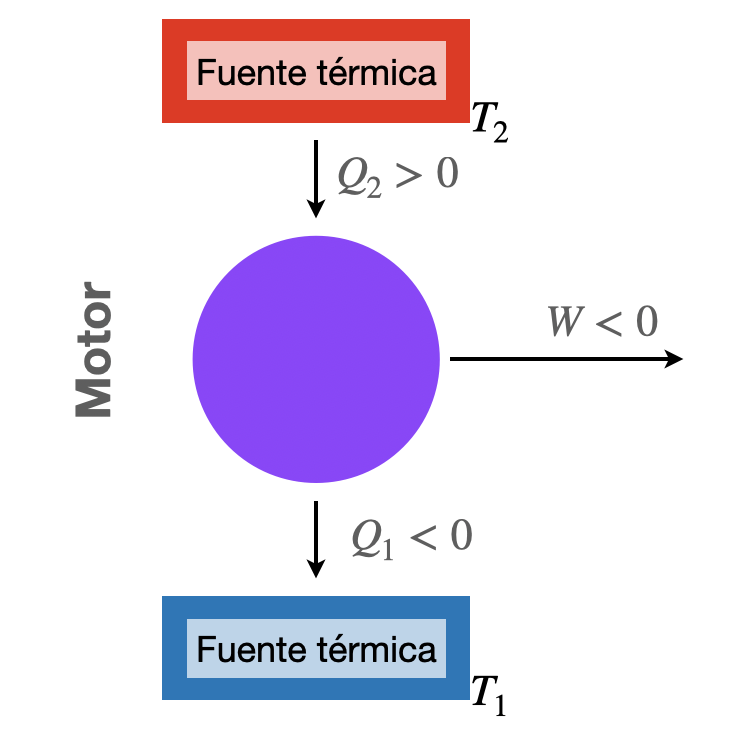
\includegraphics[width=0.87\textwidth]{img/motor_carnot.png}
    \caption{Motor}
    \label{fig:motor}
\end{figure}
\end{minipage}%
\begin{minipage}{0.5\textwidth}%
\begin{figure}[H]
    \centering
    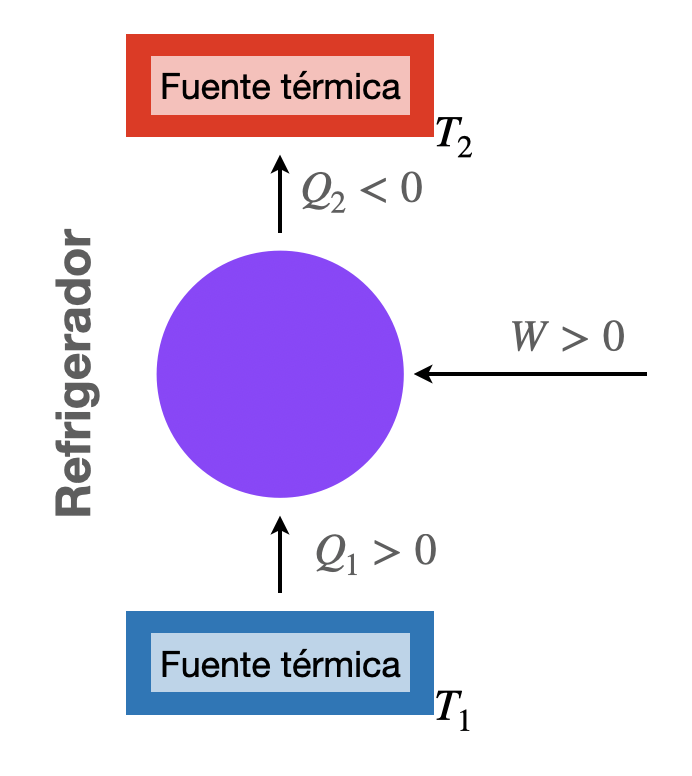
\includegraphics[width=0.79\textwidth]{img/refrigerador.png}
    \caption{Refrigerador o bomba térmica}
    \label{fig:refrigerador}
\end{figure}
\end{minipage}%
\hfill\\


Un refrigerador o bomba térmica, es un motor inverso del al cual se le inserta trabajo para aumentar la temperatura de un baño térmico \enquote{más frío}. ($W >0$)\\

\textit{La diferencia entre un refrigerador y bomba térmica recae en el uso que se le da. (Por ejemplo una bomba térmica se usa para calentar una casa en invierno, y un refrigerador para disminuir la temperatura de la comida)}\\

\textbf{Trabajo máximo:} El trabajo se maximiza para el caso reversible ($\Sigma =0$).\\

\textbf{Análisis lógico de un motor}:\label{plbr-motor}
en la ecuación $\eta = \frac{-W}{Q_2}$ se tiene que $-W$ es lo que obtenemos y $Q_2$ lo que invertimos. \textit{(Ganancia sobre inversión)}\\


\textbf{Refrigeradores - $Q_2$ y $W$}:
\label{refri-q2-w}
se tiene que en un refrigerador o bomba térmica (realizan lo mismo) se tiene la relación
\[\abs{Q_2} = (1 + \eta^R)W\]
Donde \enquote{la mejor} estufa cumple que $\abs{Q_2} = W$

\section{Ley cero de termodinámica}
% Falta información ?

Dos sistemas, cada uno por separado en equilibrio con un tercero, están en equilibrio entre sí.

\textit{Si un cuerpo ’A’ está en equilibrio con uno ’B’, y ’B’ está en equilibrio con ’C’, entonces ’A’ está en equilibrio con ’C’.}

\section{Formalismo termodinámico o potenciales termodinámicos}
\subsection{Potenciales}

\subsubsection{Variables naturales} Son las variables que si se usan para determinar cierta propiedad del sistema (S, E, F, etc) permiten obtener el resto de variables del termodinámicas del sistema.\\

Además causan que en equilibrio termodinámico, las variables definidas sean mínimas, a excepción de la entropía, que causa que sea máxima.\\

Todas las funciones (Entropía, Energía, Energía libre de Helmholtz, etc) estarán definidas en función a sus variables naturales en esta sección.\\

Si es que algunas de las funciones o su diferencial se puede expresar en relación a otras dos variables provenientes de su definición, entonces se tendrá que también serán variables naturales. (e.g. $dF = dE - TdS - SdT$, sea $dE = \gamma dA + TdS$ entonces $dF = \gamma dA - SdT$ y $F = F(A,T)$).

\subsubsection{Entropía} $S(E, V)$ es un potencial termodinámico.
\[\implies \frac{1}{T(E,V)} = \devtermo{V}{S}{E} \quad 
\land \quad \frac{p(E,V)}{T} = \devtermo{E}{S}{V}\]

\subsubsection{Energía} $E(S,V)$ es un potencial termodinámico.
\[\implies T(S,V) = \devtermo{V}{E}{S} \quad \land \quad p(S,V) = -\devtermo{S}{E}{V}\]

Teniendo en cuenta que si tenemos $S = S(T, V)$, entonces $\frac{p}{T} \neq \devtermo{T}{S}{V}$\\

\subsubsection{Energía libre de Hemholtz (o potencial, o función)} 
$F = F(T,V)=E-TS$ es un potencial termodinámico ($dE = -pdV - sdT$)

\[\implies \devtermo{T}{F}{V} = -p \quad \land \quad \devtermo{V}{F}{T} = -S\]

\subsubsection{Entalpía}
$H =H(S,p)=E+pV$ es un potencial termodinámico ($dH = TdS + Vdp$)

\[\implies \devtermo{p}{H}{S} = T \quad \land \quad \devtermo{S}{H}{p} = V\]



\subsection{Relaciones de Maxwell} 
\label{relaciones-maxwell}
Hacen uso de que los potenciales termodinámicos son de clase $\mathcal{C}^2$, por lo que sus segundas derivadas parciales con respecto a dos variables son iguales sin importar el orden de derivación. 

\begin{itemize}
    \item Para la energía:
    \[\devtermo{S}{T}{V} = -\devtermo{V}{p}{S}\]
    \item Para la energía libre de Helmholtz:
    \[\devtermo{V}{p}{T} = \devtermo{T}{S}{V}\]
    \item Para la entalpía:
    \[ \devtermo{S}{T}{p} = \devtermo{p}{V}{S} \]
\end{itemize}

\newpage % Estoy probando un sistema de jerarquía con subsecciones
%\section{Magnitudes Extensivas}

Se llama extensivas a las variables que son cuantificables y existen o son contenidas dentro del sistemas. Estas dependen de la cantidad de materia de modo que varían de forma directamente proporcional al tamaño de sistema.

\begin{itemize}
    \item Al estar contenidas en una región del espacio, se les puede asociar una densidad volumétrica.
    \item Toda magnitud extensiva es aditiva.
    \item Al trasladar un sistema, se transportan con él las magnitudes extensivas que contiene. esto permite definir corrientes.
\end{itemize}

\subsection{Magnitudes Intensivas}

En contraposición de las magnitudes extensivas están las intensivas que no dependen de la cantidad de materia, son intrínsecas.

\section{Sistemas Termodinámicos}

Se llama sistema a la región del espacio que se observa o estudia. Se distinguen tres tipos de sistemas:

\begin{itemize}
    \item \textbf{Aislado:} no intercambia magnitudes extensivas con el medio. Posee paredes adiabáticas (impiden el flujo de calor) , impermeables e inmóviles.
    \item \textbf{Cerrado:} permite en intercambio de energía con el medio. Poseen paredes diatérmicas (admiten el flujo de calor) e impermeables.
    \item \textbf{Abierto:} Permite el intercambio de energía con el medio
\end{itemize}

\subsection{Baño Térmico}

Se llama baño térmico o fuente a un sistema de tamaño mucho mayor que el del sistema de interés y que se encarga de suministrarle calor, manteniéndose a temperatura constante (su variación es despreciable).\\
Se dice que tiene capacidad calórífica o térmica ``infinita''.

\subsection{Microestados y Macroestados}

\textbf{Microestados:} distintas configuraciones que puede adoptar un sistema. El número de microestados posibles de un sistema se representa por la función $\Omega(E, N, V)$.\\

\textbf{Macroestados:} conjunto de microestados.

\subsection{Energía Interna}

La energía interna de un sistema corresponde a la suma de energía mecánica de las partículas que lo componen. Generalmente no es constante y posee una variación menor a lo medible con un instrumento típico. Se suele usar el promedio como energía interna.

\subsection{Entropía}

%Definición cualitativa de la entropía 

\textbf{Entropía de Boltzmann}

\[S(E,N,V) = k_B\ln{(\Omega(E,N,V))}\]

\subsection{Variables de Estado}

Se llama variable o función de estado a cualquier cantidad física que tiene un valor definido para cada estado de equilibrio del sistema y se puede expresar como una función de las demás variables de estado. En equilibrio térmico estas variables no dependen den tiempo, dependen sólo del estado termodinámico actual y no de como se llego hasta él.
\medbreak
Si un sistema está descrito por parámetros $x=(x_1, x_2, ...)$, para $f(x)$ una función de estado, se verifica que en un cambio de parámetros de $x_i$ a $x_f$, el cambio en $f(x)$ es

\[\Delta f = \int^{x_f}_{x_i}df = f(x_f)-f(x_i)\]

donde $df$ es un diferencial exacto, por lo que $\Delta f$ depende sólo de $x_f$ y $x_i$.

\section{Segunda Ley de la Termodinámica}
\label{2ley}
La entropía de un sistema aislado no decrece con el tiempo y es constante si y sólo si todos los procesos son reversibles.\\

También puede establecerse la segunda ley de las siguientes formas (siempre en un sistema aislado):
\begin{itemize}
    \item \textit{La entropía se puede crear, pero no se puede aniquilar}
    \item \textit{En un sistema aislado el estado de equilibrio es el de entropía máxima}
\end{itemize}

\textbf{Enunciado Microscópico:} en un sistema aislado, si se libera una restricción para las variables de estado, estas evolucionarán al valor que maximice la entropía de Boltzmann.\\

\textbf{Relación con máquinas térmicas:} \textit{NO} existe máquina térmica (motor) con rendimiento mayor al de Carnot. \label{2ley-motor}\\

\textbf{Formulación de Clausius:} no existe proceso cuyo único efecto sea transferir calor de un cuerpo frío a otro caliente.\\

\textbf{Enunciado de Kelvin:} no existe proceso cuyo único efecto sea extraer energía de un baño térmico (calor) y transformarlo en trabajo.

\section{Calor}

Flujo de energía entre cuerpos a distinta temperatura.

\subsection{Capacidad Calorífica o térmica}

Calor necesario para aumentar la temperatura de un objeto en una cierta cantidad. Es una magnitud extensiva.

\[C = \frac{dQ}{dT}\]

En baño térmico $C$ es lo suficientemente grande como para que no experimente cambios apreciables en su temperatura.

\subsection{Calor específico}

Calor necesario para aumentar la temperatura de una unidad de masa. Es una magnitud intensiva.

\[c = \frac{C}{m} = \frac{1}{m}\frac{dQ}{dT}\]

\section{Primera ley de la Termodinámica}
\label{1ley}
La energía interna de un sistema aislado es constante.

\subsection{En Términos de Calor y Trabajo}

El cambio de energía interna de un sistema $\Delta E$ es

\[\Delta E = Q+W\]

\begin{itemize}
    \item Si $Q>0$, se suministra calor al sistema y si $Q<0$ se extrae de este.
    \item Si $W>0$ se ejerce trabajo sobre el sistema y si $W<0$ el sistema ejerce trabajo sobre el medio.
    \item Para $\Delta V$ el cambio de volumen, se verifica que $w\Delta V < 0$.
\end{itemize}

\textbf{Forma Diferencial:}

\[dE = \di W+ \di Q\]

\section{Procesos Termodinámicos}

Cuando un sistema cambia de un estado de equilibrio termodinámico a otro, decimos que ocurrió un proceso.
\[(ETD)_1 \xrightarrow[]{\text{proceso}} (ETD)_2 \]

\textbf{Proceso reversible}: se definen como aquellos en donde el cambio de entropía luego de ocurrido el proceso es cero, \textit{\enquote{Se conserva la entropía}}. Un sistema que experimenta un proceso reversible es capaz de volver por sí mismo al estado original.
\\

\textbf{Proceso irreversible}: son aquellos procesos en los cuales al pasar de un (ETD) a otro existe cambio de entropía (aumenta). También se puede establecer que durante el proceso el sistema está fuera del equilibrio. Si $\Delta E_B > 0$ el proceso es irreversible. $\Sigma_r+\Sigma_d$ corresponde a la energía disipada que se va al baño y es irrecuperable.
\\

\textbf{Proceso cuasi-estático (PCE)}: si un sistema de interés va cambiando durante un proceso, de manera que a todo instante sus variables de estado están definidas (un único valor para el sistema), y se relacionan entre sí estas variables por las ecuaciones de estado, entonces decimos que el proceso es cuasi-estático. \\


En un PCE el trabajo puede ser máximo o mínimo dependiendo si es el que se extrae o el que se hace sobre el sistema.

\begin{itemize}
    \item[-] Cuando es el que se hace sobre el sistema es el trabajo mínimo paraa lograr la transformación
    \item[-] Cuando es el extraído es el máximo trabajo extraíble en la transformación. 
    
    \begin{equation}
    \begin{split}
        \text{proceso reversible} &\implies PCE\\
        &\centernot\Longleftarrow
    \end{split}
    \nonumber
\end{equation}
\end{itemize}

\textbf{Equilibrio para un sistema}: cuando sus variables de estado (\textit{S, E, N, V, p, T, ...}) se relacionan por las ecuaciones de estado.\\

\textit{Dos fronteras están en equilibrio entre sí, si $T_1 = T_2$ cuando la pared es diatérmica, o si $p_1 = p_2$ cuando la pared es móvil.}

\subsection{Ciclos}
\label{ciclos}
Un ciclo es una serie proceso en el que se regresa al estado inicial (esto no implica que sean reversibles).\\

\textbf{Ciclo de Carnot:} Ciclo reversible que reversible que involucra 2 baños térmicos en el que se repiten los siguientes procesos:

\begin{itemize}
    \item En contacto con el baño 2 se aumenta la entropía de $S_1$ a $S_2$
    \item En un proceso adiabático ($\Delta S=0$) se baja la temperatura de $T_2$ a $T_1$
    \item En contacto con el baño 1 se disminuya la entropía de $S_2$ a $S_1$
    \item En un proceso adiabático se aumenta la temperatura de $T_1$ a $T_2$
\end{itemize}

El ciclo de Carnot recorrido en este sentido constituye un motor que minimiza la energía disipada y maximiza el trabajo extraído. Recorrido en el sentido inverso forma un refrigerador.

\begin{itemize}
    \item \textbf{Temperaturas absolutas:} el ciclo se Carnot permite definir temperaturas independientes del sistema. Se fija una temperatura $T_2$, y se define $T_1$ como
\[T_1 = T_2(1-\eta_c)\]
\end{itemize}

\subsection{Motores}

En un motor se realiza un ciclo con dos baños térmico, uno caliente y otro frío, que permite extraer trabajo ($W<0$).\\

\begin{minipage}{0.5\textwidth}%
\begin{figure}[H]
    \centering
    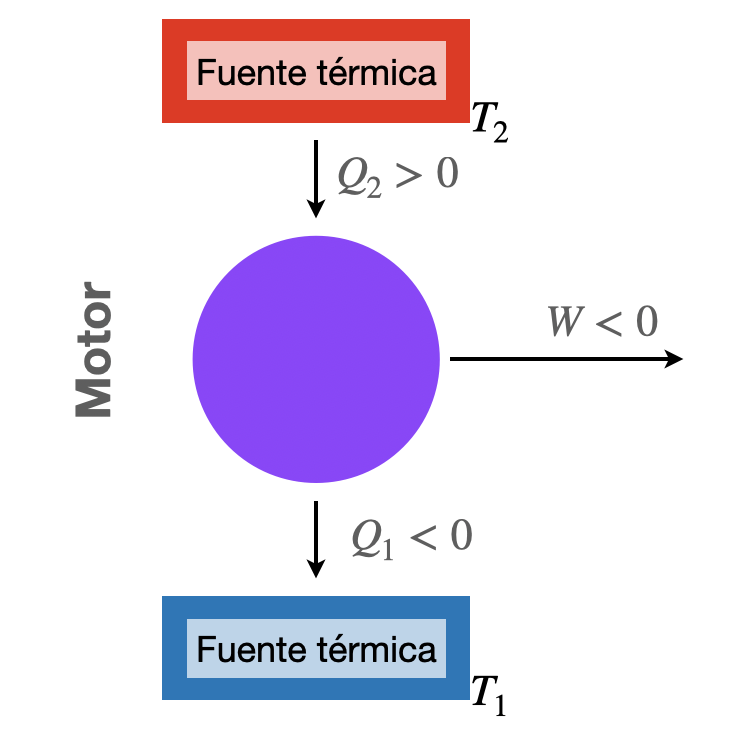
\includegraphics[width=0.87\textwidth]{img/motor_carnot.png}
    \caption{Motor}
    \label{fig:motor}
\end{figure}
\end{minipage}%
\begin{minipage}{0.5\textwidth}%
\begin{figure}[H]
    \centering
    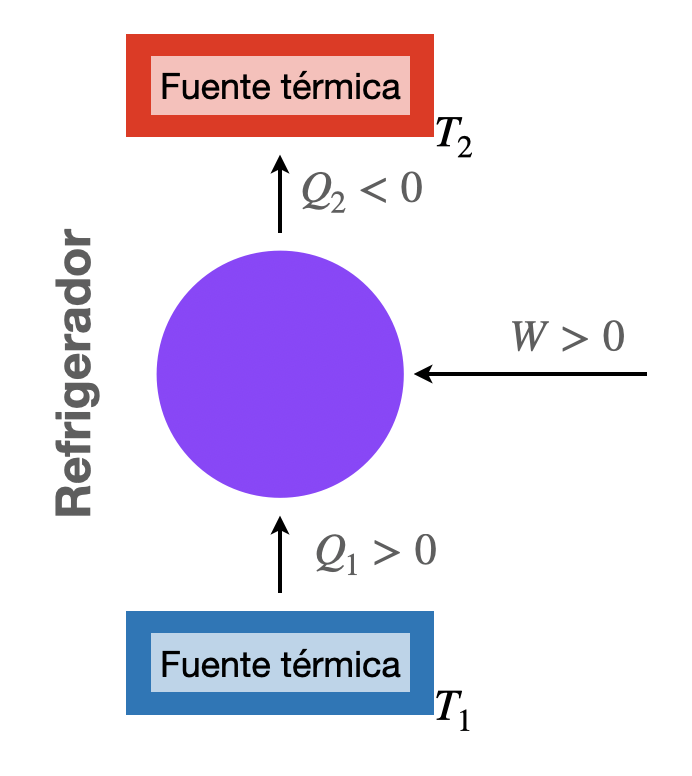
\includegraphics[width=0.79\textwidth]{img/refrigerador.png}
    \caption{Refrigerador o bomba térmica}
    \label{fig:refrigerador}
\end{figure}
\end{minipage}%
\hfill\\

Un refrigerador o bomba térmica, es un motor inverso del al cual se le inserta trabajo para aumentar la temperatura de un baño térmico \enquote{más frío}. ($W >0$)\\

\textbf{Análisis lógico de un motor}:\label{plbr-motor}
en la ecuación $\eta = \frac{-W}{Q_2}$ se tiene que $W$ es lo que queremos obtener y $Q_2$ lo que invertimos.\\

\textbf{Refrigeradores - $Q_2$ y $W$}:
\label{refri-q2-w}
se tiene que en un refrigerador o bomba térmica (realizan lo mismo) se tiene la relación
\[\abs{Q_2} = (1 + \eta^R)W\]
Donde \enquote{la mejor} estufa cumple que $\abs{Q_2} = W$

\section{Ley cero de termodinámica}
% Falta información ?

Dos sistemas, cada uno por separado en equilibrio con un tercero, están en equilibrio entre sí.

\textit{Si un cuerpo ’A’ está en equilibrio con uno ’B’, y ’B’ está en equilibrio con ’C’, entonces ’A’ está en equilibrio con ’C’.}

\section{Formalismo termodinámico o potenciales termodinámicos}

\textbf{Entropía}: $S(E, V)$ es un potencial termodinámico.
\[\implies \frac{1}{T(E,V)} = \devtermo{V}{S}{E} \quad 
\land \quad \frac{p(E,V)}{T} = \devtermo{E}{S}{V}\]

\textbf{Energía}: $E(S,V)$ es un potencial termodinámico.
\[\implies T(S,V) = \devtermo{V}{E}{S} \quad \land \quad p(S,V) = -\devtermo{S}{E}{V}\]

Teniendo en cuenta que si tenemos $S = S(T, V)$, entonces $\frac{p}{T} \neq \devtermo{T}{S}{V}$\\

\textbf{Variables naturales}: son las variables que si se usan para determinar cierta propiedad del sistema (S, E, F, etc) permiten obtener el resto de variables del termodinámicas del sistema.\\

Además causan que en equilibrio termodinámico, las variables definidas sean mínimas, a excepción de la entropía, que causa que sea máxima.\\

Todas las funciones (Entropía, Energía, Energía libre de Helmholtz, etc) estarán definidas en función a sus variables naturales en esta sección.\\

Si es que algunas de las funciones o su diferencial se puede expresar en relación a otras dos variables provenientes de su definición, entonces se tendrá que también serán variables naturales. (e.g. $dF = dE - TdS - SdT$, sea $dE = \gamma dA + TdS$ entonces $dF = \gamma dA - SdT$ y $F = F(A,T)$).\\

\textbf{Energía libre de Hemholtz (o potencial, o función)}: $F = F(T,V)=E-TS$ es un potencial termodinámico ($dE = -pdV - sdT$)

\[\implies \devtermo{T}{F}{V} = -p \quad \land \quad \devtermo{V}{F}{T} = -S\]

\textbf{Entalpía}: $H =H(S,p)=E+pV$ es un potencial termodinámico ($dH = TdS + Vdp$)

\[\implies \devtermo{p}{H}{S} = T \quad \land \quad \devtermo{S}{H}{p} = V\]



\textbf{Relaciones de Maxwell}: \label{relaciones-maxwell} hacen uso de que los potenciales termodinámicos son de clase $\mathcal{C}^2$, por lo que sus segundas derivadas parciales con respecto a dos variables son iguales sin importar el orden de derivación. 

\begin{itemize}
    \item Para la energía:
    \[\devtermo{S}{T}{V} = -\devtermo{V}{p}{S}\]
    \item Para la energía libre de Helmholtz:
    \[\devtermo{V}{p}{T} = \devtermo{T}{S}{V}\]
    \item Para la entalpía:
    \[ \devtermo{S}{T}{p} = \devtermo{p}{V}{S} \]
\end{itemize}

\newpage
\section{Justificaciones y Demostraciones}

\subsection{Definición estadística de la temperatura}
\label{DTemperatura}
Si se consideran dos sistemas aislados que admiten el traspaso de energía con microestados $\Omega_1 = \Omega(E_1, N_1, V_1)$ y $\Omega_2 = \Omega(E_2, N_2, V_2)$, el sistema formado por ambos tiene $\Omega_1\Omega_2$ microestados y energía interna $E = E_1+E_2$ constante. Con el tiempo suficiente se llegará al equilibrio térmico, en donde se maximiza $\Omega_1\Omega_2$

\[\frac{d}{dE_1}(\Omega_1\Omega_2)=
\Omega_2\frac{d\Omega_1}{dE_1} + 
\Omega_1\frac{d\Omega_2}{dE_2}\frac{dE_2}{dE_1}=0\]

como $E$ es constante

\[\frac{dE}{dE_1}=1+\frac{dE_2}{dE_1}=0
\Rightarrow \frac{dE_2}{dE_1}=-1\]

\begin{equation}
\begin{split}
    \frac{1}{\Omega_1}\frac{d\Omega_1}{dE_1}-
    \frac{1}{\Omega_2}\frac{d\Omega_2}{dE_2}=0
    & \Rightarrow \frac{d\ln{(\Omega_1)}}{dE_1} =
    \frac{d\ln{(\Omega_2)}}{dE_2}\\
    & \Rightarrow \frac{dS(E_1,N_1,V_1)}{dE_1} =
    \frac{dS(E_2,N_2,V_2)}{dE_2}\\
\end{split}
\nonumber
\end{equation}

A esta condición se le dice \enquote{estar a igual temperatura} y se usa para definir la temperatura por la ecuación

\[\frac{1}{T}=\frac{dS}{dE}\]

\subsection{Capacidad Calorífica en equilibrio}
\label{Cequilibrio}

Por primera ley se tiene que

\[\di Q = dE - \di W\]

y en equilibrio térmico $\di W = -pdV$, considerando que la energía interna es función de la temperatura y el volumen, $E(T,V)$, se tiene que

\begin{equation}
\begin{split}
    C &= \frac{dQ}{dT}\\
    &= \frac{dE}{dT}+p\frac{dV}{dT}\\
    &= \devtermo{V}{E}{T}+\devtermo{T}{E}{V}\frac{dV}{dT}+
    p\frac{dV}{dT}\\
    &=\devtermo{V}{E}{T}+\lados{[}{\devtermo{T}{E}{V}+p}\frac{dV}{dT}\\
\end{split}
\nonumber
\end{equation}
Si se mantiene $p$ constante, se obtiene
\[C_p = \devtermo{V}{E}{T}+\lados{[}{\devtermo{T}{E}{V}+p}\devtermo{p}{V}{T}\]


\subsection{Cambio nulo de temperatura}
\label{DT=0}
Si las temperaturas inicial y final de un proceso son iguales ($\Delta T = 0$), se tiene que

\begin{equation}
\begin{split}
    \Delta T = 0 &\Rightarrow \Delta E = 0\\
    &\Rightarrow W=-Q\\
    &\Rightarrow \Delta S = \Sigma - \frac{W}{T}\\
    &\Rightarrow T(\Sigma-\Delta S)\\
\end{split}
\nonumber
\end{equation}

Dado que $\Sigma \geq 0$, se cumple también que $W\geq -T\Delta S$.

\subsection{Trabajo y calor en ciclos}
\label{TQciclos}
\textbf{1 baño:}

\begin{equation}
\begin{split}
    &\Delta E = Q + W = 0 \Rightarrow Q = -W\\
    &W = \Delta E - T(\Delta S-\Sigma) = T\Sigma\\
\end{split}
\nonumber
\end{equation}

\textbf{2 baños:}

\begin{equation}
\begin{split}
    &\Delta E = Q_1 + Q_2 + W \Rightarrow W = -Q_1-Q_2\\
    &\Delta S = \Sigma+\frac{Q_1}{T_1}+\frac{Q_2}{T_2}
    \Rightarrow Q_1 = -\lados{(}{\frac{T_1}{T_2}Q_2+T_1\Sigma}\\
\end{split}
\nonumber
\end{equation}

\subsection{Trabajo de un motor de Carnot}
\label{TCarnot}
La magnitud del trabajo de un ciclo de Carnot es igual al área encerrada por la curva que describe en el plano $TS$ y su signo esta dado según la orientación en que se recorre el ciclo.

\begin{equation}
\begin{split}
    0<(T_2-T_1)(S_2-S_1) &= (T_2-T_1)\frac{Q_2}{T_2}\\
    &=Q_2-\frac{T_1}{T_2}Q_2\\
    &=Q_2+Q_1\\
    &=-W\\
\end{split}
\nonumber
\end{equation}

\newpage
% Esta puede ser la de datos 'random', si no creamos un otro archivo

\section{Misceláneo}

Se hará uso de la siguiente notación:
	\begin{itemize}
	    \item $k_B$ o $K_B$: constante de Boltzmann
	    \item \textit{N}: cantidad de moléculas en un sistema a estudiar
	    \item \textit{p}: presión
	    \item \textit{V}: volumen
	    \item \textit{E}: energía interna de un sistema
	    \item \textit{S}: entropía
	    \item $S_B$: entropía de un baño térmico
	    \item \textit{T}: temperatura (medida en Kelvin) (siempre $ T \geq 0$)
	    \item \textit{C}: capacidad calórica
	    \item $C_V$: capacidad calórica a volumen constante
	    \item $C_p$: capacidad calórica a presión constante
	    \item \textit{c}: calor específico
	    \item \textit{Q}: calor entregado \textit{al} sistema
	    
	    En caso de dos baños térmicos se tiene usualmente que:
	    \begin{itemize}
	        \item $Q_1$ es el baño \enquote{frío} 
	        \item $Q_2$ es el baño \enquote{caliente}
	    \end{itemize}
	    Ambos tienen temperaturas mayor a cero, pero $T_1 < T_2$
	    
	    \item \textit{W}: trabajo hecho \textit{sobre} el sistema
	\end{itemize}

\subsection{Fórmula de Stirling}

\[\ln n! \approx n\ln ( n )- n\]

\subsection{Mucha presión}

Si se ejerce una presión sobre un sistema mucho mayor a su presión interna, el sistema está fuera de equilibrio y por tanto no existe una única temperatura que lo caracterice.

\subsection{\textit{E(S,N,V)}}
\label{eq:e(s,v,n)}
Como al inicio del curso se tiene que $N$ es constante, entonces esto equivale a $E(S,V)$. Donde se obtiene $E$ a partir de la ecuación de Sackur-Tetrode y es para gases ideales monoatómicos.

\[ E(S,N,V) = \frac{3N}{4 \pi m}\lados{(}{\frac{Nh^3}{V}}^{(2/3)}\exp\lados{[}{\frac{2S}{3Nk_B} - \frac{5}{3}} \]

\subsection{Ciclo de Carnot en imágenes}
A la izquierda corresponde a un diagrama \textit{p-V} y el de la derecha a uno \textit{S-T}.

\begin{figure}[H]
    \centering
    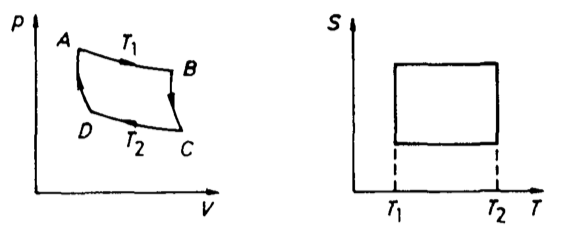
\includegraphics[width=0.65\textwidth]{img/ciclo_carnot.png}
    \caption{Diagrama ciclo de Carnot}
    \label{fig:diag_carnot}
\end{figure}

\subsection{Diferencial de Entalpía}

\[dH = C_pdT - \lados{[}{T\devtermo{p}{V}{T} - V}dp\]

\subsection{Relación cíclica}
\label{sub:relacion_ciclica}
Sea $z = z(x, y) \in \mathcal{C}^n$, con $n \geq 2$ entonces se tiene que:

\[\devtermo{y}{z}{x}\devtermo{z}{x}{y}\devtermo{x}{y}{z} = -1\]

\subsection{Coeficientes de expansión}

\begin{itemize}
    \item Coeficiente de expansión isotérmica
    \[ \beta \equiv -\devtermo{T}{V}{p}\frac{1}{V} \]
    
    \item Coeficiente de expansión térmica
    \[ \alpha \equiv \devtermo{p}{V}{T}\frac{1}{V} \]
\end{itemize}

\begin{equation}
\begin{split}
    \implies C_p &= C_V - T\devtermo{p}{V}{T}\devtermo{V}{p}{T}\\
                 &= C_V + TV\frac{\alpha^2}{\beta} 
\end{split}
\nonumber
\end{equation}

\end{document}
